\section{Introduction to Languages}
Front End languages are language that are used to give better user experince and user interface. These mainly include HTML, CSS, PHP. Some Frameworks like Bootstrap are also used with these basic languages.
\subsection{HTML}

\begin{figure}[h]
\centering 
\includegraphics[scale=0.05]{images/HTML.png}
\caption{HTML5 logo}
\end{figure}
HyperText Markup Language, commonly referred to as HTML, is the standard markup language used to create web pages. Along with CSS, and HTML is a cornerstone technology, used by most websites to create visually engaging webpages, user interfaces for web applications, and user interfaces for many mobile applications. \\
Web browsers can read HTML files and render them into visible or audible web pages. HTML describes the structure of a website semantically along with cues for presentation, making it a markup language, rather than a programming language.\\
HTML elements form the building blocks of all websites. HTML allows images and objects to be embedded and can be used to create interactive forms. It provides a means to create structured documents by denoting structural semantics for text such as headings, paragraphs, lists, links, quotes and other items.


\subsection{CSS}

\begin{figure}[h]
\centering 
\includegraphics[scale=0.50]{images/CSS.jpg}
\caption{CSS logo}
\end{figure}
Cascading Style Sheets (CSS) is a style sheet language used for describing the presentation of a document written in a markup language.Although most often used to set the visual style of web pages and user interfaces written in HTML and XHTML, the language can be applied to any XML document, including plain XML, SVG and XUL, and is applicable to rendering in speech, or on other media. \\
Along with HTML and JavaScript, CSS is a cornerstone technology used by most websites to create visually engaging webpages, user interfaces for web applications, and user interfaces for many mobile applications.\\
CSS is designed primarily to enable the separation of document content from document presentation, including aspects such as the layout, colors, and fonts.\\
 This separation can improve content accessibility, provide more flexibility and control in the specification of presentation characteristics, enable multiple HTML pages to share formatting by specifying the relevant CSS in a separate .css file, and reduce complexity and repetition in the structural content, such as semantically insignificant tables that were widely used to format pages before consistent CSS rendering was available in all major browsers.\\
 CSS makes it possible to separate presentation instructions from the HTML content in a separate file or style section of the HTML file. For each matching HTML element, it provides a list of formatting instructions

\subsection{PHP}
\begin{figure}[h!]
\centering 
\includegraphics[scale=0.50]{images/php.png}
\caption{PHP logo}
\end{figure}
 {\bf What is PHP?}
\begin{itemize}
   \item  PHP is an acronym for "PHP: Hypertext Preprocessor"
    \item PHP is a widely-used, open source scripting language
     \item PHP scripts are executed on the server
     \item  PHP is free to download and use\\
\end{itemize}
 {\bf What is a PHP File?}
\begin{itemize}
     \item PHP files can contain text, HTML, CSS, JavaScript, and PHP code
    \item PHP code are executed on the server, and the result is returned to the browser as plain HTML
    \item  PHP files have extension ".php"\\
\end{itemize}
 {\bf What Can PHP Do?}

  \begin{itemize}
    \item PHP can generate dynamic page content
    \item PHP can create, open, read, write, delete, and close files on the server
     \item PHP can collect form data
     \item PHP can send and receive cookies
    \item  PHP can add, delete, modify data in your database
    \item PHP can be used to control user-access
     \item PHP can encrypt data\\
\end{itemize}
  {\bf Why PHP?}
 \begin{itemize}
 \item   PHP runs on various platforms (Windows, Linux, Unix, Mac OS X, etc.)
 \item   PHP is compatible with almost all servers used today (Apache, IIS, etc.)
\item    PHP supports a wide range of databases
 \item   PHP is free. Download it from the official PHP resource: www.php.net
 \item   PHP is easy to learn and runs efficiently on the server side
\end{itemize}





\section{Introduction to CGS}
\textbf{\emph{User Manual}}\\\\
It could also deal with CSV Format. CSV(Character Separated File) is a simple file format used to store tabular data, such as a
spreadsheet or database. Files in the CSV format can be imported to and exported from programs
that store data in tables, such as Microsoft Excel or OpenOffice CAs the Name "Certificate Generation System" Implies this application is used to 
generate certificate in an automated manner in few steps: 
\begin{enumerate}
\item Select Design from the images shown on the first page.
   (Put mouse pointer over the image to see larger view.)
\begin{figure}[!ht]
\centering
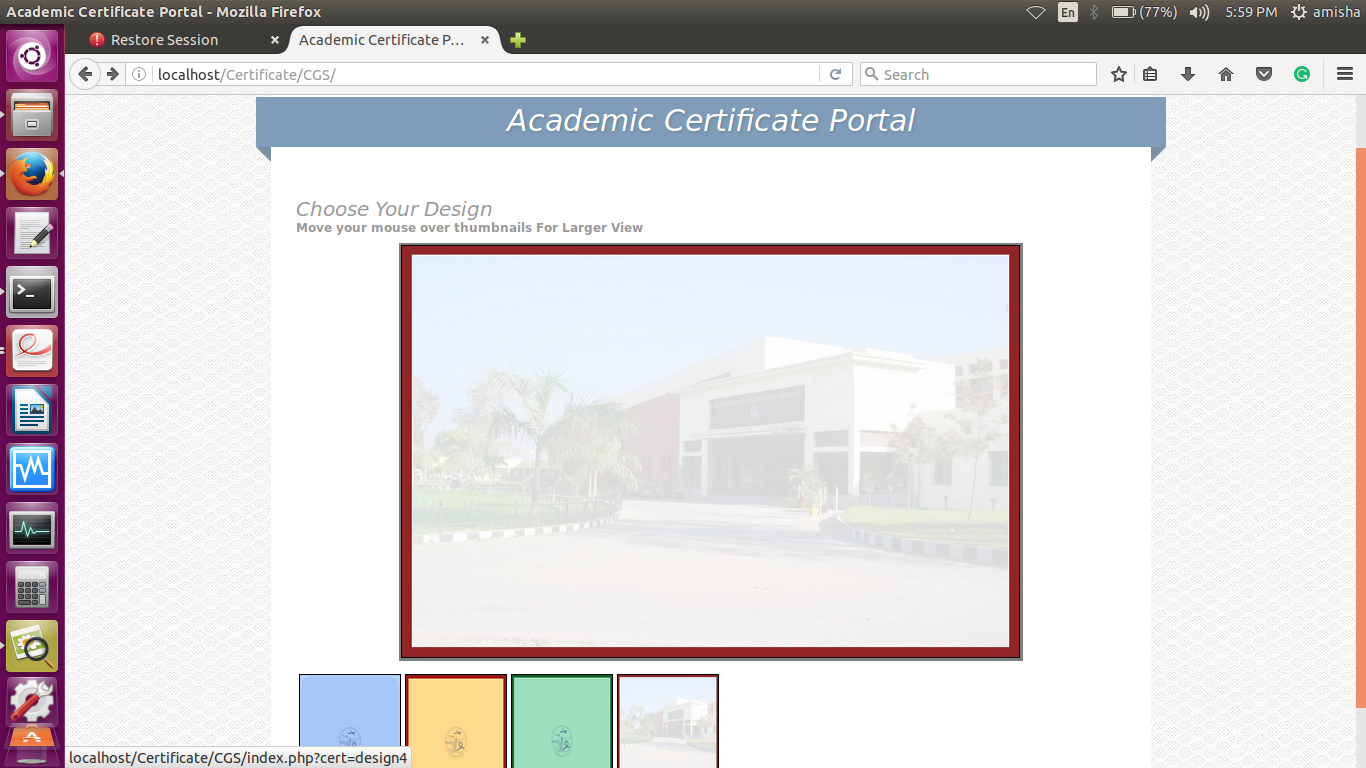
\includegraphics[width=0.85\textwidth]{images/cgs/cgs1.png}
\caption{Academic Portal}
\hspace{-1.5em}
\end{figure}
\item Next Page will be page for entering College Details.
\begin{itemize}
\item Fill in the details of institution for which the certificate(s) is to be made.
\begin{figure}[!ht]
\centering
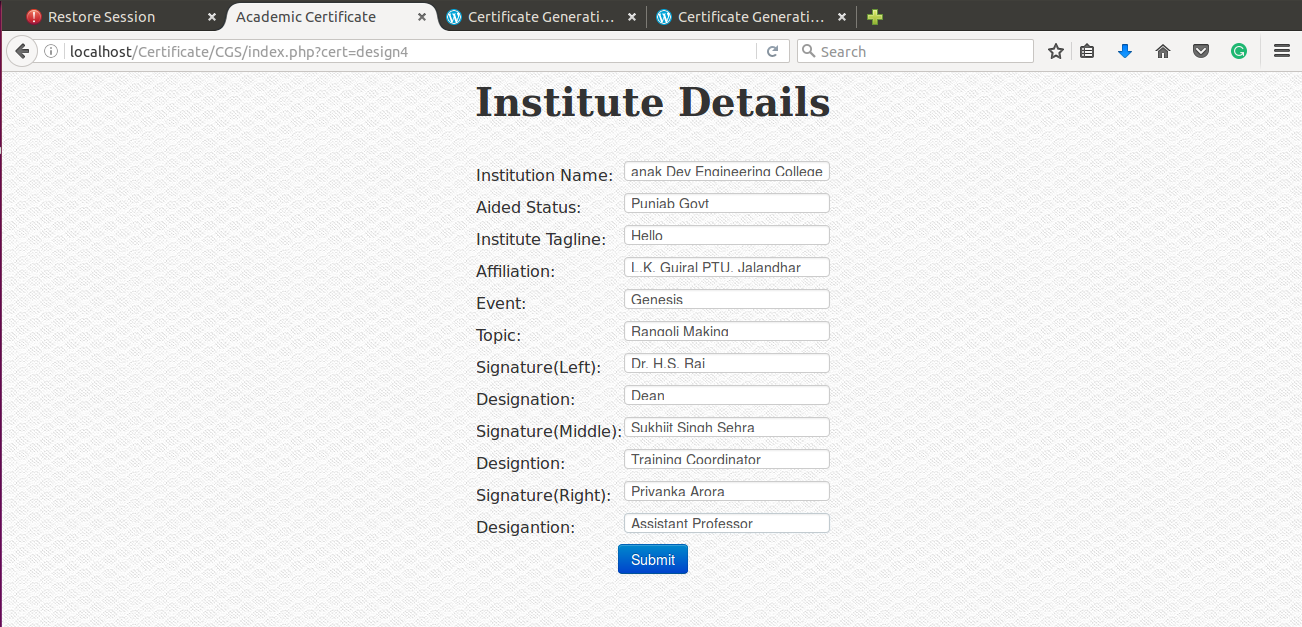
\includegraphics[width=0.85\textwidth]{images/cgs/cgs2.png}                  
\caption{Institute Details}
\hspace{-1.5em}
\end{figure}
\item Place mouse pointer over Input box te see an example for that input.
\end{itemize}
\item Next page will show two options
\begin{itemize}
\item Manual Entry    -> Select it for Generating Certificate for Single candidate.
\item Upload Csv File -> Select it for Generating certificate for more than 1 candidate by providing their details in Csv file.
\begin{figure}[!ht]
\centering
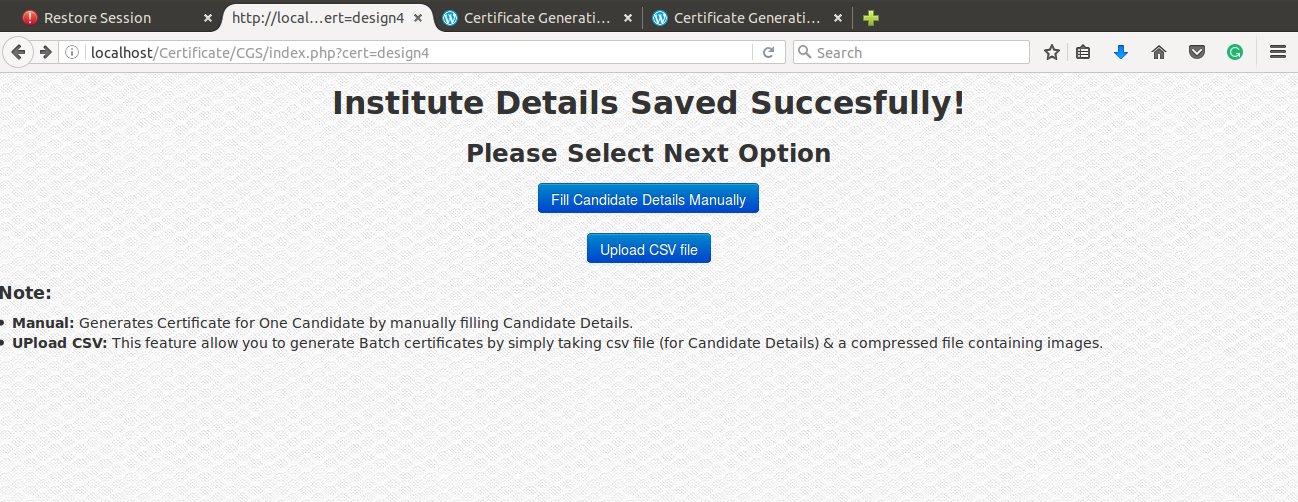
\includegraphics[width=0.85\textwidth]{images/cgs/cgs3.png}                  
\caption{Select Manual Option}
\hspace{-1.5em}
\end{figure}
\end{itemize}
\end{enumerate}

\section{Installation and Setup}
\textbf{\emph{Manual Filling}}
\begin{itemize}
\item On Selecting Manual Entry Next page will open containing input boxes for candidate Details.
\item Enter the details and select the image also.
\end{itemize}
Also by clicking on "Generate Another Ceritificate" you can generate another certificate with same design \& institute details and different Candidate Details.
And by clicking on "Goto First Page" you can again start from Design Selection Page.\\\\
\begin{itemize}
\item On Selecting Manual Entry Next page will open containing input boxes for candidate Details.
\item Enter the details and select the image also.
\item Live Image Selector
\item Next you will be displayed your selected image and a selection box.

\begin{figure}[!ht]
\centering
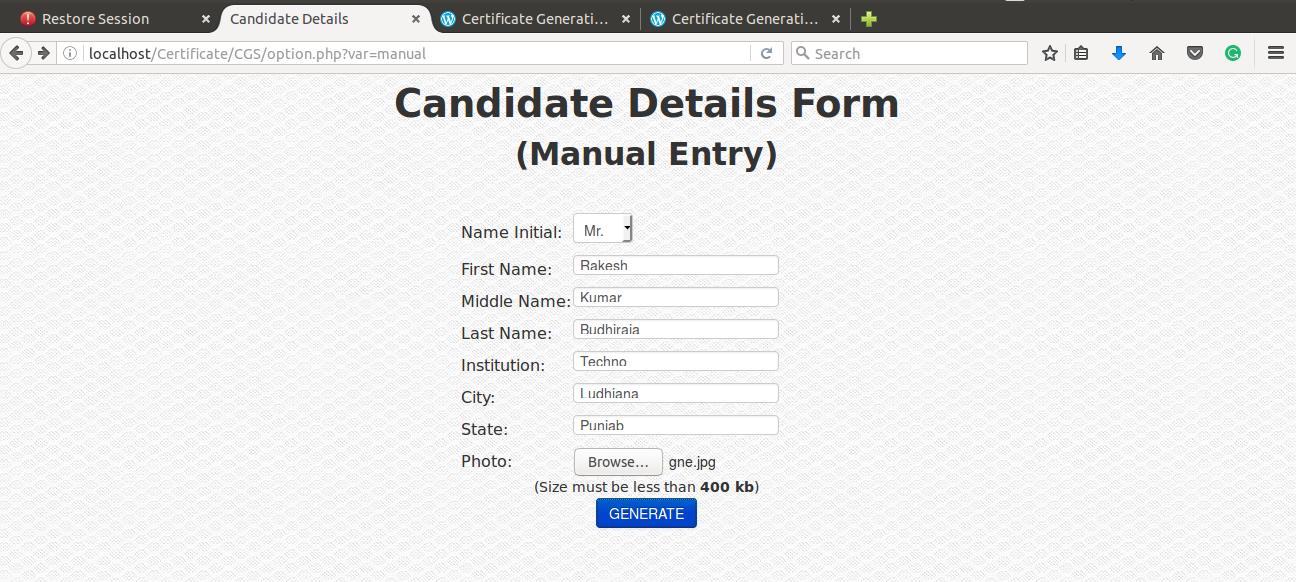
\includegraphics[width=0.85\textwidth]{images/cgs/cgs4.png}                  
\caption{Candidate Details Form}
\hspace{-1.5em}
\end{figure}

\item Resize and move the selection box to desired position and size.

\begin{figure}[!ht]
\centering
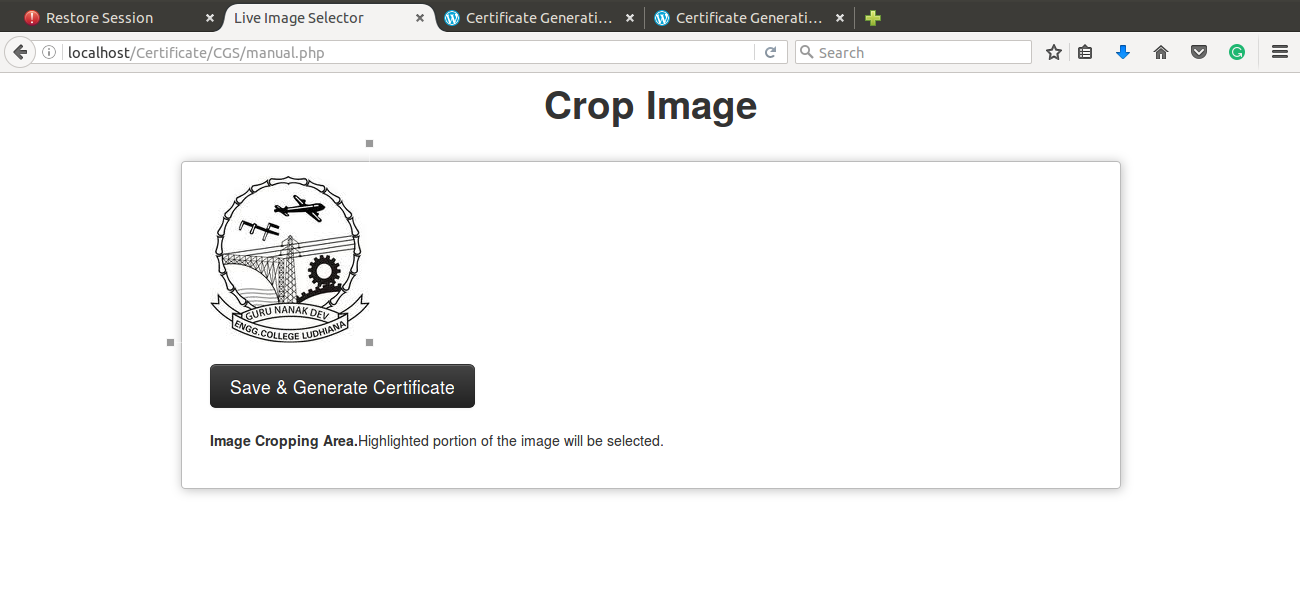
\includegraphics[width=0.85\textwidth]{images/cgs/cgs5.png}                  
\caption{Crop Image}
\hspace{-1.5em}
\end{figure}
\end{itemize}
\newpage
\textbf{\emph{Csv Format}}
\begin{enumerate}
\item On selecting 'Upload csv File' Next page will open containing the conditions for the files to be uploaded for certificate generation.
\item A sample file can be downloaded from the link provided in the 'Note' in the instructions on page.
\item Sample file is a zip file named sample.zip containing the csv file and .zip file for images.
\item Extract it and then sample certificates can be produced using 'sample.csv' and 'images.zip' files.
\item That's it your certificate file is produced for all the candidates provided in the csv data file.
\end{enumerate}  
\newpage
\textbf{\emph{Download}}\\\\
That's it your certificate file is produced for all the candidates provided in the csv data file.\\
The final result i.e Certificate can be saved in more than one format:
\begin{itemize}
\item pdf (portable document format)
\item Any other format eg. odt etc.
\end{itemize}
\begin{figure}[!ht]
\centering
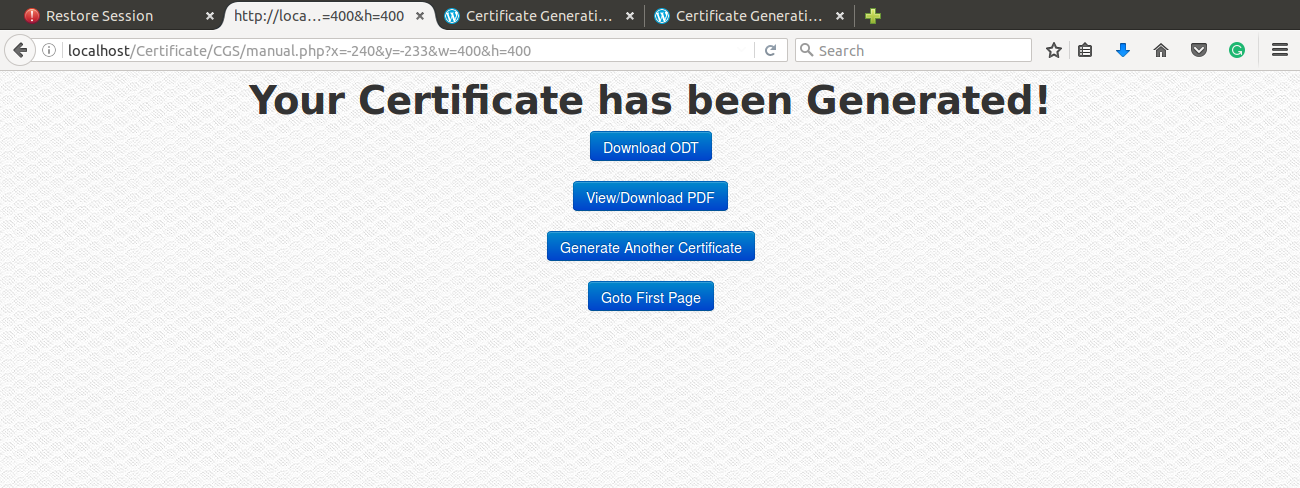
\includegraphics[width=0.85\textwidth]{images/cgs/cgs6.png}                  
\caption{Download Certificate}
\hspace{-1.5em}
\end{figure}
\begin{figure}[!ht]
\centering
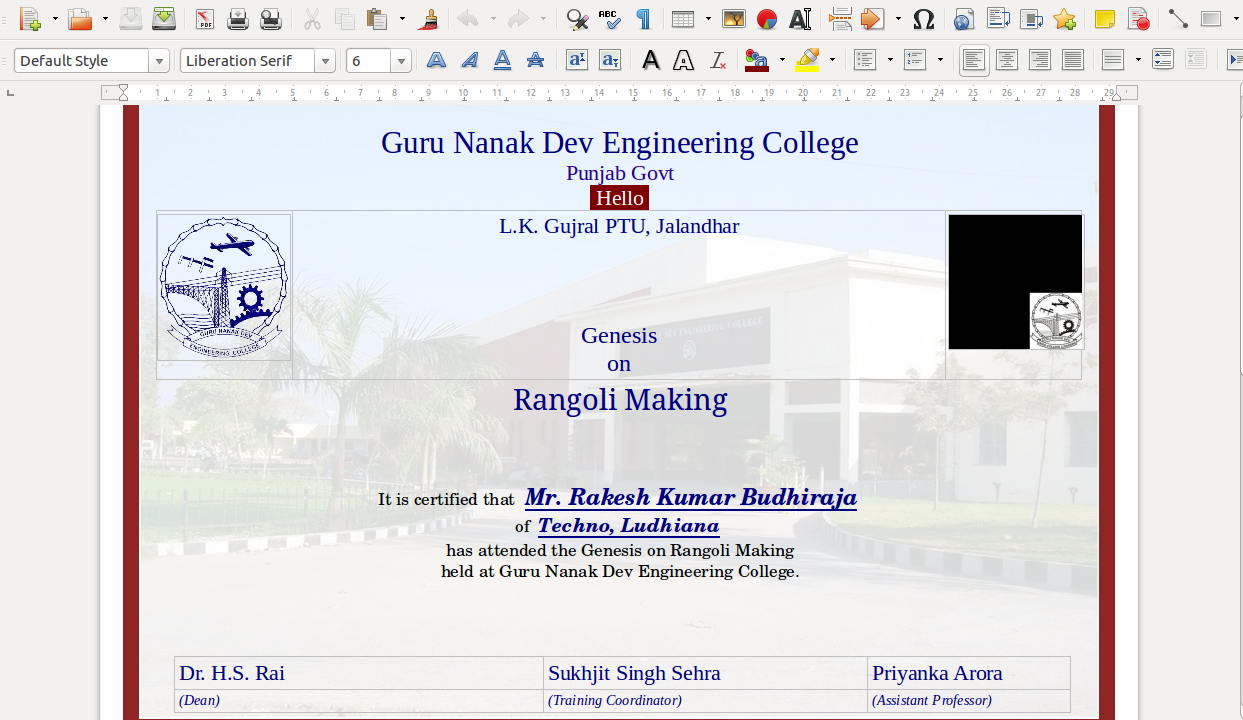
\includegraphics[width=0.85\textwidth]{images/cgs/cgs8.png}                 
\caption{Certificate odt file}
\hspace{-1.5em}
\end{figure}
\begin{figure}[!ht]
\centering
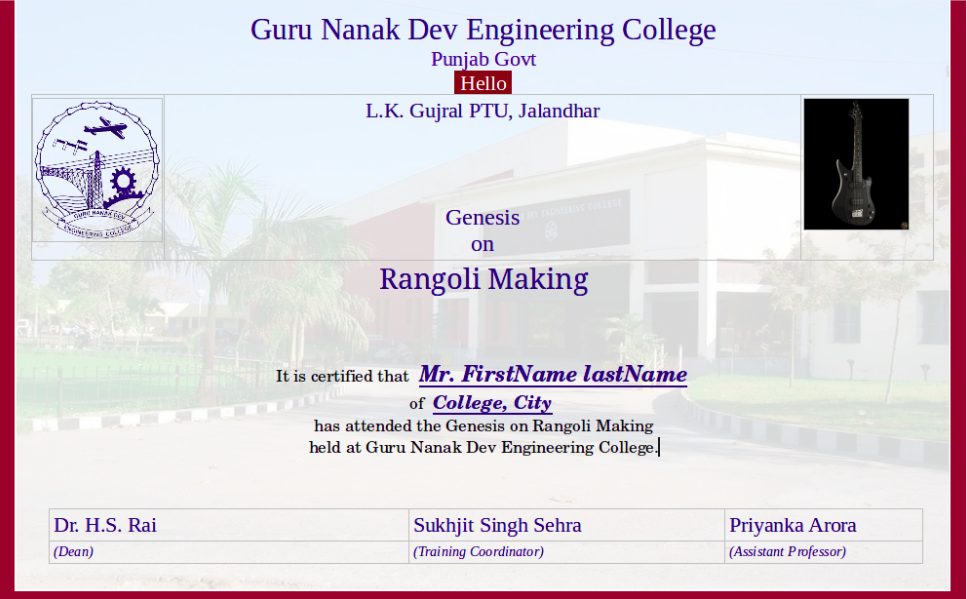
\includegraphics[width=0.85\textwidth]{images/cgs/pdf.png}
\caption{Certificate pdf file}
\hspace{-1.5em}
\end{figure}
Next page will open containing the conditions for the files to be uploaded for certificate generation.
\begin{figure}[!ht]
\centering
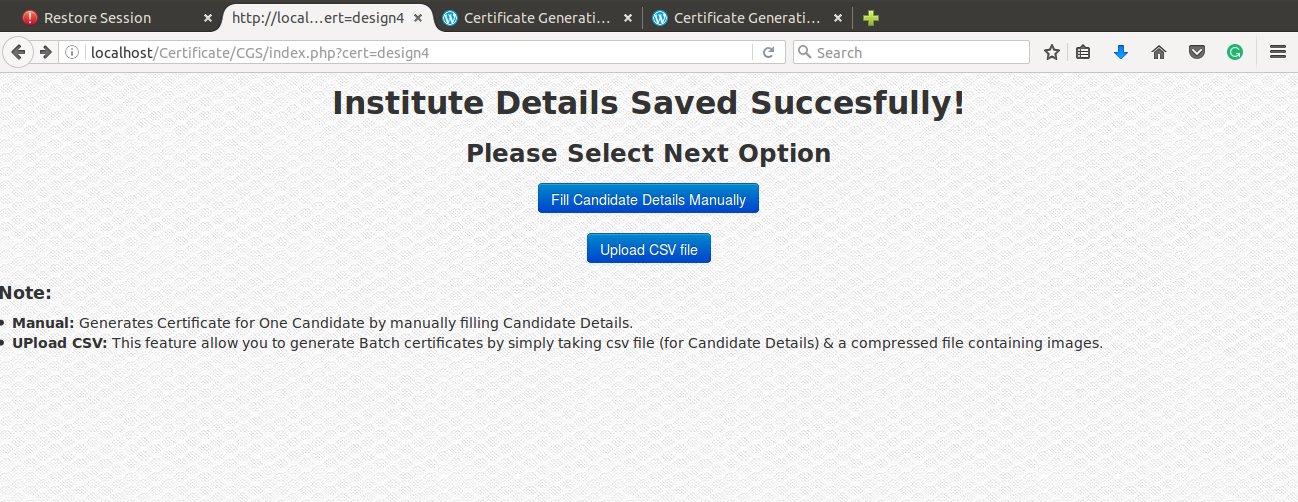
\includegraphics[width=0.85\textwidth]{images/cgs/cgs3.png}                  
\caption{Choose csv Option}
\hspace{-1.5em}
\end{figure}
A sample file can be downloaded from the link provided in the 'Note' in the instructions on page. Sample file is a zip file named sample.zip containing the csv file and tar.gz file for images.\\\\
Extract it and then sample certificates can be produced using 'sample.csv' and 'images.tar.gz' files.

\begin{figure}[!ht]
\centering
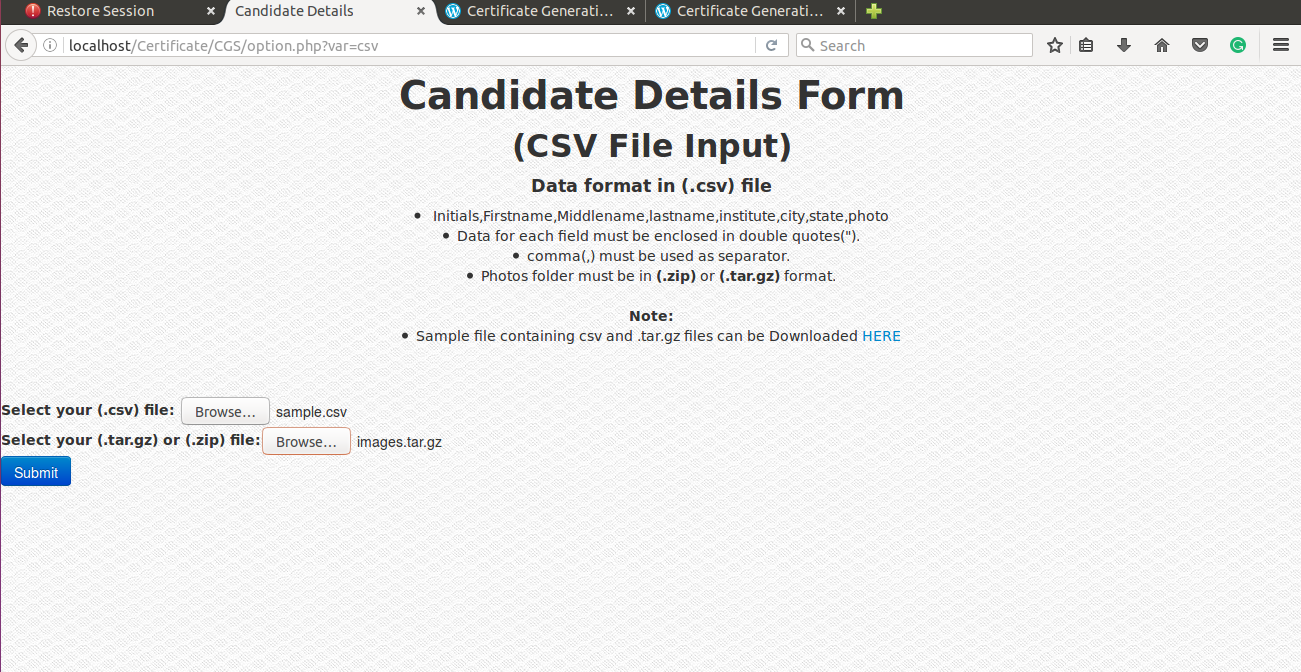
\includegraphics[width=0.85\textwidth]{images/cgs/cgs9.png}                 
\caption{Candidate Details Form}
\hspace{-1.5em}
\end{figure}
-> odt ('O'penOffice 'D'ocument 'T'ext)\\
-> pdf ('P'ortable 'D'ocument 'F'ormat)\\
The result of the csv file certificates are like below:\\
These certificates sizes can be arranged accordingly.\\

\begin{figure}[ht!]
\centering
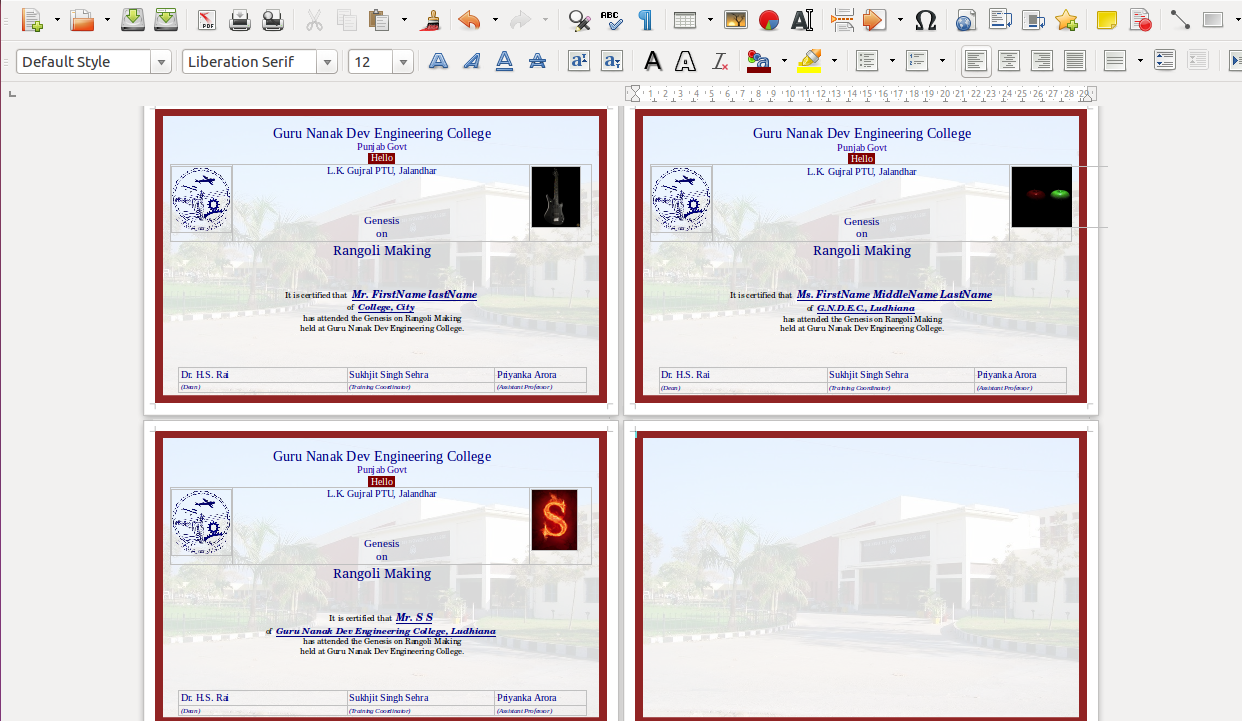
\includegraphics[width=0.85\textwidth]{images/cgs/cgs14.png}                  
\caption{Odt file through csv}
\hspace{-1.5em}
\end{figure}




